% Generated by Sphinx.
\def\sphinxdocclass{report}
\documentclass[letterpaper,10pt,english]{sphinxmanual}
\usepackage[utf8]{inputenc}
\DeclareUnicodeCharacter{00A0}{\nobreakspace}
\usepackage{cmap}
\usepackage[T1]{fontenc}
\usepackage{babel}
\usepackage{times}
\usepackage[Bjarne]{fncychap}
\usepackage{longtable}
\usepackage{sphinx}
\usepackage{multirow}

\addto\captionsenglish{\renewcommand{\figurename}{Fig. }}
\addto\captionsenglish{\renewcommand{\tablename}{Table }}
\floatname{literal-block}{Listing }



\title{QuantHoop Documentation}
\date{October 14, 2015}
\release{1.0}
\author{Hao Lin}
\newcommand{\sphinxlogo}{}
\renewcommand{\releasename}{Release}
\makeindex

\makeatletter
\def\PYG@reset{\let\PYG@it=\relax \let\PYG@bf=\relax%
    \let\PYG@ul=\relax \let\PYG@tc=\relax%
    \let\PYG@bc=\relax \let\PYG@ff=\relax}
\def\PYG@tok#1{\csname PYG@tok@#1\endcsname}
\def\PYG@toks#1+{\ifx\relax#1\empty\else%
    \PYG@tok{#1}\expandafter\PYG@toks\fi}
\def\PYG@do#1{\PYG@bc{\PYG@tc{\PYG@ul{%
    \PYG@it{\PYG@bf{\PYG@ff{#1}}}}}}}
\def\PYG#1#2{\PYG@reset\PYG@toks#1+\relax+\PYG@do{#2}}

\expandafter\def\csname PYG@tok@gd\endcsname{\def\PYG@tc##1{\textcolor[rgb]{0.63,0.00,0.00}{##1}}}
\expandafter\def\csname PYG@tok@gu\endcsname{\let\PYG@bf=\textbf\def\PYG@tc##1{\textcolor[rgb]{0.50,0.00,0.50}{##1}}}
\expandafter\def\csname PYG@tok@gt\endcsname{\def\PYG@tc##1{\textcolor[rgb]{0.00,0.27,0.87}{##1}}}
\expandafter\def\csname PYG@tok@gs\endcsname{\let\PYG@bf=\textbf}
\expandafter\def\csname PYG@tok@gr\endcsname{\def\PYG@tc##1{\textcolor[rgb]{1.00,0.00,0.00}{##1}}}
\expandafter\def\csname PYG@tok@cm\endcsname{\let\PYG@it=\textit\def\PYG@tc##1{\textcolor[rgb]{0.25,0.50,0.56}{##1}}}
\expandafter\def\csname PYG@tok@vg\endcsname{\def\PYG@tc##1{\textcolor[rgb]{0.73,0.38,0.84}{##1}}}
\expandafter\def\csname PYG@tok@m\endcsname{\def\PYG@tc##1{\textcolor[rgb]{0.13,0.50,0.31}{##1}}}
\expandafter\def\csname PYG@tok@mh\endcsname{\def\PYG@tc##1{\textcolor[rgb]{0.13,0.50,0.31}{##1}}}
\expandafter\def\csname PYG@tok@cs\endcsname{\def\PYG@tc##1{\textcolor[rgb]{0.25,0.50,0.56}{##1}}\def\PYG@bc##1{\setlength{\fboxsep}{0pt}\colorbox[rgb]{1.00,0.94,0.94}{\strut ##1}}}
\expandafter\def\csname PYG@tok@ge\endcsname{\let\PYG@it=\textit}
\expandafter\def\csname PYG@tok@vc\endcsname{\def\PYG@tc##1{\textcolor[rgb]{0.73,0.38,0.84}{##1}}}
\expandafter\def\csname PYG@tok@il\endcsname{\def\PYG@tc##1{\textcolor[rgb]{0.13,0.50,0.31}{##1}}}
\expandafter\def\csname PYG@tok@go\endcsname{\def\PYG@tc##1{\textcolor[rgb]{0.20,0.20,0.20}{##1}}}
\expandafter\def\csname PYG@tok@cp\endcsname{\def\PYG@tc##1{\textcolor[rgb]{0.00,0.44,0.13}{##1}}}
\expandafter\def\csname PYG@tok@gi\endcsname{\def\PYG@tc##1{\textcolor[rgb]{0.00,0.63,0.00}{##1}}}
\expandafter\def\csname PYG@tok@gh\endcsname{\let\PYG@bf=\textbf\def\PYG@tc##1{\textcolor[rgb]{0.00,0.00,0.50}{##1}}}
\expandafter\def\csname PYG@tok@ni\endcsname{\let\PYG@bf=\textbf\def\PYG@tc##1{\textcolor[rgb]{0.84,0.33,0.22}{##1}}}
\expandafter\def\csname PYG@tok@nl\endcsname{\let\PYG@bf=\textbf\def\PYG@tc##1{\textcolor[rgb]{0.00,0.13,0.44}{##1}}}
\expandafter\def\csname PYG@tok@nn\endcsname{\let\PYG@bf=\textbf\def\PYG@tc##1{\textcolor[rgb]{0.05,0.52,0.71}{##1}}}
\expandafter\def\csname PYG@tok@no\endcsname{\def\PYG@tc##1{\textcolor[rgb]{0.38,0.68,0.84}{##1}}}
\expandafter\def\csname PYG@tok@na\endcsname{\def\PYG@tc##1{\textcolor[rgb]{0.25,0.44,0.63}{##1}}}
\expandafter\def\csname PYG@tok@nb\endcsname{\def\PYG@tc##1{\textcolor[rgb]{0.00,0.44,0.13}{##1}}}
\expandafter\def\csname PYG@tok@nc\endcsname{\let\PYG@bf=\textbf\def\PYG@tc##1{\textcolor[rgb]{0.05,0.52,0.71}{##1}}}
\expandafter\def\csname PYG@tok@nd\endcsname{\let\PYG@bf=\textbf\def\PYG@tc##1{\textcolor[rgb]{0.33,0.33,0.33}{##1}}}
\expandafter\def\csname PYG@tok@ne\endcsname{\def\PYG@tc##1{\textcolor[rgb]{0.00,0.44,0.13}{##1}}}
\expandafter\def\csname PYG@tok@nf\endcsname{\def\PYG@tc##1{\textcolor[rgb]{0.02,0.16,0.49}{##1}}}
\expandafter\def\csname PYG@tok@si\endcsname{\let\PYG@it=\textit\def\PYG@tc##1{\textcolor[rgb]{0.44,0.63,0.82}{##1}}}
\expandafter\def\csname PYG@tok@s2\endcsname{\def\PYG@tc##1{\textcolor[rgb]{0.25,0.44,0.63}{##1}}}
\expandafter\def\csname PYG@tok@vi\endcsname{\def\PYG@tc##1{\textcolor[rgb]{0.73,0.38,0.84}{##1}}}
\expandafter\def\csname PYG@tok@nt\endcsname{\let\PYG@bf=\textbf\def\PYG@tc##1{\textcolor[rgb]{0.02,0.16,0.45}{##1}}}
\expandafter\def\csname PYG@tok@nv\endcsname{\def\PYG@tc##1{\textcolor[rgb]{0.73,0.38,0.84}{##1}}}
\expandafter\def\csname PYG@tok@s1\endcsname{\def\PYG@tc##1{\textcolor[rgb]{0.25,0.44,0.63}{##1}}}
\expandafter\def\csname PYG@tok@gp\endcsname{\let\PYG@bf=\textbf\def\PYG@tc##1{\textcolor[rgb]{0.78,0.36,0.04}{##1}}}
\expandafter\def\csname PYG@tok@sh\endcsname{\def\PYG@tc##1{\textcolor[rgb]{0.25,0.44,0.63}{##1}}}
\expandafter\def\csname PYG@tok@ow\endcsname{\let\PYG@bf=\textbf\def\PYG@tc##1{\textcolor[rgb]{0.00,0.44,0.13}{##1}}}
\expandafter\def\csname PYG@tok@sx\endcsname{\def\PYG@tc##1{\textcolor[rgb]{0.78,0.36,0.04}{##1}}}
\expandafter\def\csname PYG@tok@bp\endcsname{\def\PYG@tc##1{\textcolor[rgb]{0.00,0.44,0.13}{##1}}}
\expandafter\def\csname PYG@tok@c1\endcsname{\let\PYG@it=\textit\def\PYG@tc##1{\textcolor[rgb]{0.25,0.50,0.56}{##1}}}
\expandafter\def\csname PYG@tok@kc\endcsname{\let\PYG@bf=\textbf\def\PYG@tc##1{\textcolor[rgb]{0.00,0.44,0.13}{##1}}}
\expandafter\def\csname PYG@tok@c\endcsname{\let\PYG@it=\textit\def\PYG@tc##1{\textcolor[rgb]{0.25,0.50,0.56}{##1}}}
\expandafter\def\csname PYG@tok@mf\endcsname{\def\PYG@tc##1{\textcolor[rgb]{0.13,0.50,0.31}{##1}}}
\expandafter\def\csname PYG@tok@err\endcsname{\def\PYG@bc##1{\setlength{\fboxsep}{0pt}\fcolorbox[rgb]{1.00,0.00,0.00}{1,1,1}{\strut ##1}}}
\expandafter\def\csname PYG@tok@mb\endcsname{\def\PYG@tc##1{\textcolor[rgb]{0.13,0.50,0.31}{##1}}}
\expandafter\def\csname PYG@tok@ss\endcsname{\def\PYG@tc##1{\textcolor[rgb]{0.32,0.47,0.09}{##1}}}
\expandafter\def\csname PYG@tok@sr\endcsname{\def\PYG@tc##1{\textcolor[rgb]{0.14,0.33,0.53}{##1}}}
\expandafter\def\csname PYG@tok@mo\endcsname{\def\PYG@tc##1{\textcolor[rgb]{0.13,0.50,0.31}{##1}}}
\expandafter\def\csname PYG@tok@kd\endcsname{\let\PYG@bf=\textbf\def\PYG@tc##1{\textcolor[rgb]{0.00,0.44,0.13}{##1}}}
\expandafter\def\csname PYG@tok@mi\endcsname{\def\PYG@tc##1{\textcolor[rgb]{0.13,0.50,0.31}{##1}}}
\expandafter\def\csname PYG@tok@kn\endcsname{\let\PYG@bf=\textbf\def\PYG@tc##1{\textcolor[rgb]{0.00,0.44,0.13}{##1}}}
\expandafter\def\csname PYG@tok@o\endcsname{\def\PYG@tc##1{\textcolor[rgb]{0.40,0.40,0.40}{##1}}}
\expandafter\def\csname PYG@tok@kr\endcsname{\let\PYG@bf=\textbf\def\PYG@tc##1{\textcolor[rgb]{0.00,0.44,0.13}{##1}}}
\expandafter\def\csname PYG@tok@s\endcsname{\def\PYG@tc##1{\textcolor[rgb]{0.25,0.44,0.63}{##1}}}
\expandafter\def\csname PYG@tok@kp\endcsname{\def\PYG@tc##1{\textcolor[rgb]{0.00,0.44,0.13}{##1}}}
\expandafter\def\csname PYG@tok@w\endcsname{\def\PYG@tc##1{\textcolor[rgb]{0.73,0.73,0.73}{##1}}}
\expandafter\def\csname PYG@tok@kt\endcsname{\def\PYG@tc##1{\textcolor[rgb]{0.56,0.13,0.00}{##1}}}
\expandafter\def\csname PYG@tok@sc\endcsname{\def\PYG@tc##1{\textcolor[rgb]{0.25,0.44,0.63}{##1}}}
\expandafter\def\csname PYG@tok@sb\endcsname{\def\PYG@tc##1{\textcolor[rgb]{0.25,0.44,0.63}{##1}}}
\expandafter\def\csname PYG@tok@k\endcsname{\let\PYG@bf=\textbf\def\PYG@tc##1{\textcolor[rgb]{0.00,0.44,0.13}{##1}}}
\expandafter\def\csname PYG@tok@se\endcsname{\let\PYG@bf=\textbf\def\PYG@tc##1{\textcolor[rgb]{0.25,0.44,0.63}{##1}}}
\expandafter\def\csname PYG@tok@sd\endcsname{\let\PYG@it=\textit\def\PYG@tc##1{\textcolor[rgb]{0.25,0.44,0.63}{##1}}}

\def\PYGZbs{\char`\\}
\def\PYGZus{\char`\_}
\def\PYGZob{\char`\{}
\def\PYGZcb{\char`\}}
\def\PYGZca{\char`\^}
\def\PYGZam{\char`\&}
\def\PYGZlt{\char`\<}
\def\PYGZgt{\char`\>}
\def\PYGZsh{\char`\#}
\def\PYGZpc{\char`\%}
\def\PYGZdl{\char`\$}
\def\PYGZhy{\char`\-}
\def\PYGZsq{\char`\'}
\def\PYGZdq{\char`\"}
\def\PYGZti{\char`\~}
% for compatibility with earlier versions
\def\PYGZat{@}
\def\PYGZlb{[}
\def\PYGZrb{]}
\makeatother

\renewcommand\PYGZsq{\textquotesingle}

\begin{document}

\maketitle
\tableofcontents
\phantomsection\label{index::doc}


Contents:


\chapter{What is QuantHoops}
\label{_static/basic:what-is-quanthoops}\label{_static/basic::doc}\label{_static/basic:welcome-to-quanthoop-s-documentation}
There is a revolution happening in basketball. The convergence of technology,
data and forward thinking basketball minds has produced a new wave of statistical
analysis. With the help of new technology, data that was once tracked in secret,
behind NBA walls, is now available for the masses.

At the collegiate level, there are thousands of hard data points, but most programs
don't know what to do with all the information. There aren't many programs
maximizing the data currently at their fingertips, and we are going to change that.

For a college basketball coach, it is easy to become overwhelmed with the amount
of data available (if you are even looking at it). You most likely don't have
the budget to hire a full-time Director of Basketball Analytics. With this
site, you won't have to. We can do the work for you.

Our hope is to highlight key trends in the data for both self scouting and
opponent analysis. What do the numbers mean? How do the advanced stats translate
on film? What am I seeing on paper to validate/refute my assumptions about our
team or our opponents? What are the key takeaways?

If you are a college coach in D1, D2 or D3, let QuantHoops become your outsourced,
high-powered Basketball Analytics departments.


\section{What we do}
\label{_static/basic:what-we-do}
We provide deep analysis by triangulating available data points like tempo-free
stats, synergy analytics, SportVU data and video breakdown; time of possession,
efficiency by play type, and possession ratings. This stuff is all done at the
NBA level, but hardly seen in the college ranks... The list is limitless.

Our goal is to highlight key trends in data for both self-scouting and opponent
analysis and roll it into an easily digestible format, including:
\begin{itemize}
\item {} 
In-season game by game analysis

\item {} 
In-season opponent scouting reports

\item {} 
5 man unit analysis and position combinations

\item {} 
Player profiles and individual analysis

\item {} 
End of season self-scouting reports (team and players)

\item {} 
Synergy statistical analysis

\item {} 
SportVU data analysis

\end{itemize}


\section{Tempo-Free Philosophy}
\label{_static/basic:tempo-free-philosophy}
Points per possessions and points allowed per possession are two of the most
important stats in basketball. How often do you score, how often do you get
stops? Every coach must know where his/her team stands across each of these
categories, right?

Wrong.

This seems like a mainstream concept, yet why are tempo-free stats still so
under-utilized? How many coaches know their team’s average points per possession?
And what about other tempo-free stats? How many know their turnovers rate (TOs
per possession)? How many coaches look at the numbers, yet don’t know what to
do with them?

In Division 1, these stats are readily available. You can trend, slice and
dice this data for days. As an example, most D1 teams license Synergy scouting
software, primarily for film exchange and video scouts. Most users don’t utilize
the volume of data Synergy houses by team, player, conference, play-type, etc.

If you wanted to, you could literally run tempo-free reports all day. But more
importantly, what should you do with all this data? Triangulating these data
points – tempo-free stats, synergy analytics and video breakdown, can be a
powerful tool for any program. Unfortunately, very few programs have the time
and resources to effectivelly use this information.

In a perfect world, most schools would hire a Director of Basketball Analytics
to track and analyze things like five-man unit data (points per possession,
pts allowed per possession for each unit), position combinations, time of
possession, efficiency by play type, possession ratings, track shot location,
player efficiency by play type, individual defensive (forced shot missed,
allowed field goal). The list is almost endless.

At the D2 and D3 levels, tempo-free stats were up to this point nonexistent.
Not anymore my friends. Want to know the most efficient team in the NESCAC
conference? Who’s the worst defensive team in all of D2? Look no further folks,
this site is your answer.

If nothing else, it can’t hurt to look at this data. With the help of a trained
eye (QuantHoops), we’ll help you find the value hidden in the numbers.


\section{Contact}
\label{_static/basic:contact}
\href{mailto:Info@quanthoops.com}{Info@quanthoops.com}

Tel: (781) 420-9019


\chapter{Database design}
\label{_static/database::doc}\label{_static/database:database-design}
The database is designed based on \href{http://stats.ncaa.org/}{stats.ncaa.org}


\section{Season table}
\label{_static/database:season-table}
Use ncaa\_id to determine season and gender, no matter what the division is.

The data entry must be manually inserted into table, because we can not predict
the season\_id that ncaa will use for the next season. Men and Women will use
same season\_id for the same season.

Table structure:

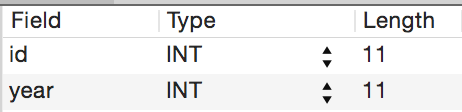
\includegraphics{season_table.png}

Table content (until season 2014/2015):

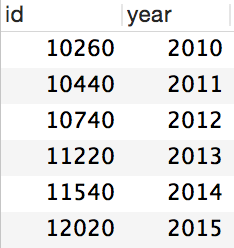
\includegraphics{season_content.png}


\section{Conference table}
\label{_static/database:conference-table}
A team may belong to different conference in different year and division.

So conference will have one-to-one maps to Squad.

Table structure:

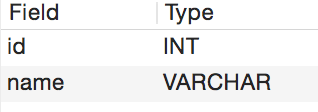
\includegraphics{conference_table.png}


\section{Team table}
\label{_static/database:team-table}
Teams contain a relationship to Squads for any available years.
Also contain relationships to alternate team names.

NCAA uses a permanent id (org\_id, which is also known as ncaa\_id)to
represent a team no matter what the season is.

Note that IDs have been assigned explicitly to match those used by
NCAA.com to make record linkage easier. The alternate team names
and fuzzy matching capabilities are just in case another source is
used.

One-to-many maps to Squads.

Table structure:

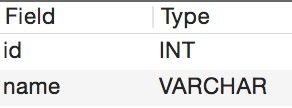
\includegraphics{team_table.png}


\section{Squad table}
\label{_static/database:squad-table}
Squads contain basic information of a Team in a given season.

One-to-many maps to SquadMembers, Games. Many-to-one map to Team.

Table structure:

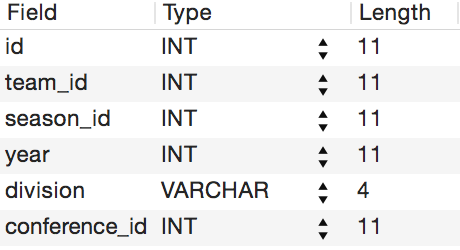
\includegraphics{squad_table.png}


\section{Schedule table}
\label{_static/database:schedule-table}
One game will have two schedules for both team, indicate which one is
home team, and which one is away team.

NCAA will post all schedules for the whole season, and fill the game
details when match is complete.

Table structure:

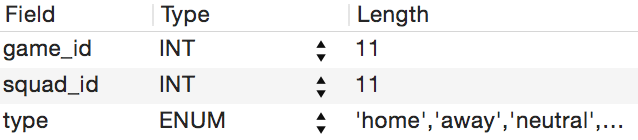
\includegraphics{schedule_table.png}


\section{Game table}
\label{_static/database:game-table}
Game holds references to two Squads. Holds a collection of total score,
first \& second half score, first \& second overtime score.
Allow for specification of winner and loser.
Also hold vital statistics such as where and when and attendance.

Many-to-many map to Squads via Schedule, one-to-many map to PlayerGameStat.

Table structure:

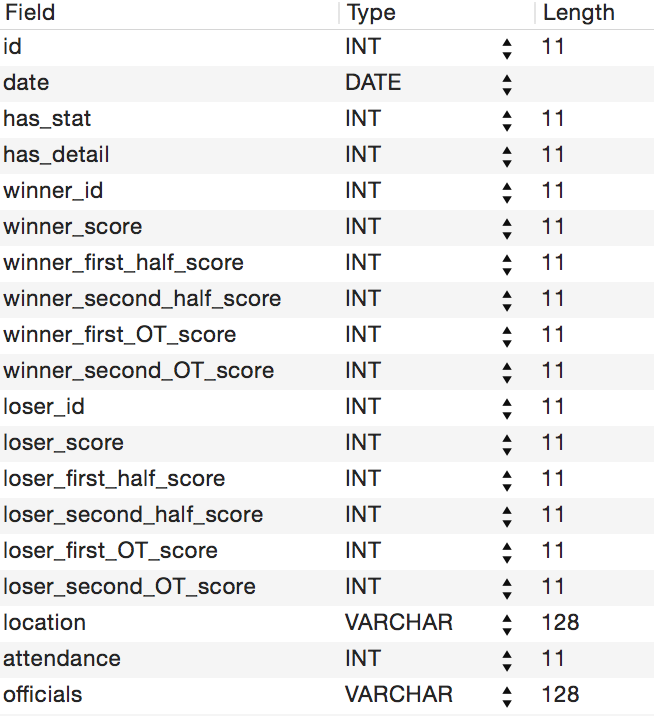
\includegraphics{game_table.png}


\section{Player table}
\label{_static/database:player-table}
Players possess a one-to-many mapping to SquadMembers,
which are essentially chrono-sensitive versions of the Player. For
example, a Player's corresponding SquadMember from 2010-11 will not
have access to that Player's statistics from 2011-12, nor will these
latest statistics be incorporated into the earlier SquadMember's record.
This allows for more realistic simulations.

Table structure:

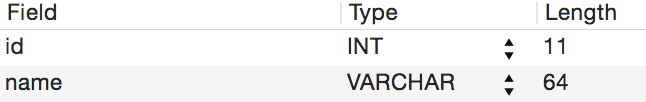
\includegraphics{player_table.png}


\section{SquadMember table}
\label{_static/database:squadmember-table}
This is the class that holds Player's basic information.
Many-to-one maps to Player, Squad, and Game

Table structure:

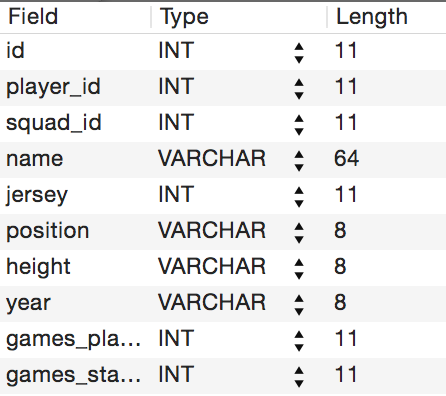
\includegraphics{squadmember_table.png}


\section{PlayerSeasonStat table}
\label{_static/database:playerseasonstat-table}
Contains the stats of one SquadMember in one Season

Many-to-one maps to SquadMember

Table structure:

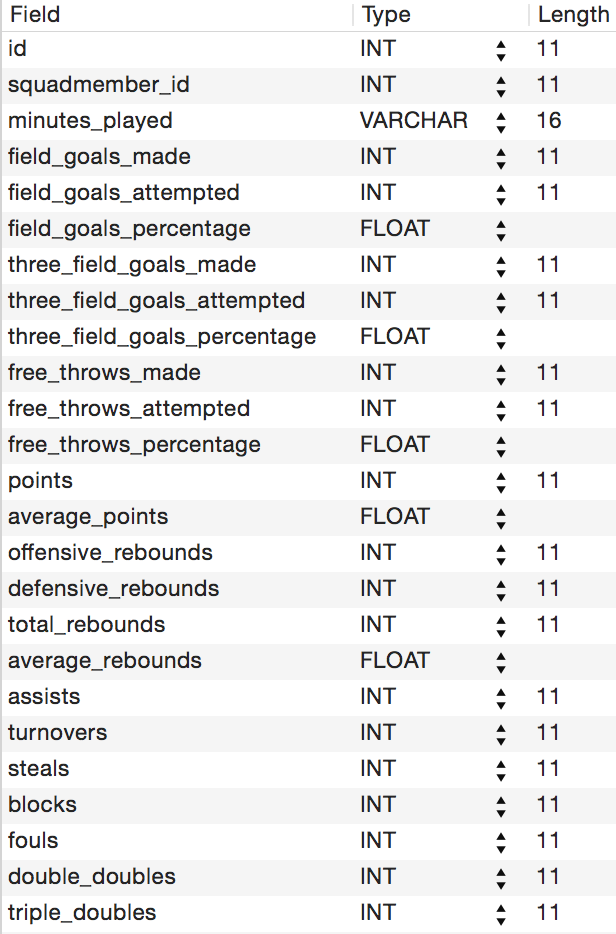
\includegraphics{PlayerSeasonStat_table.png}


\section{SquadSeasonStat table}
\label{_static/database:squadseasonstat-table}
Contains the stats of one Squad in one Season.

one-to-one maps to Squad.

Table structure:

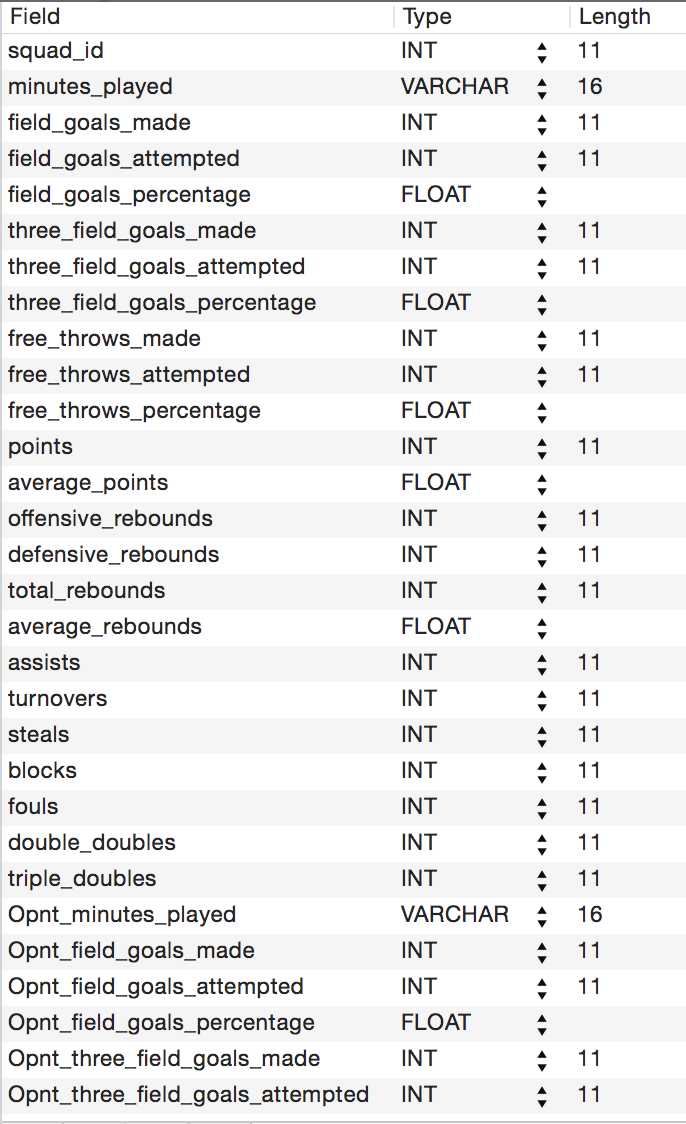
\includegraphics{SquadSeasonStat_table1.png}

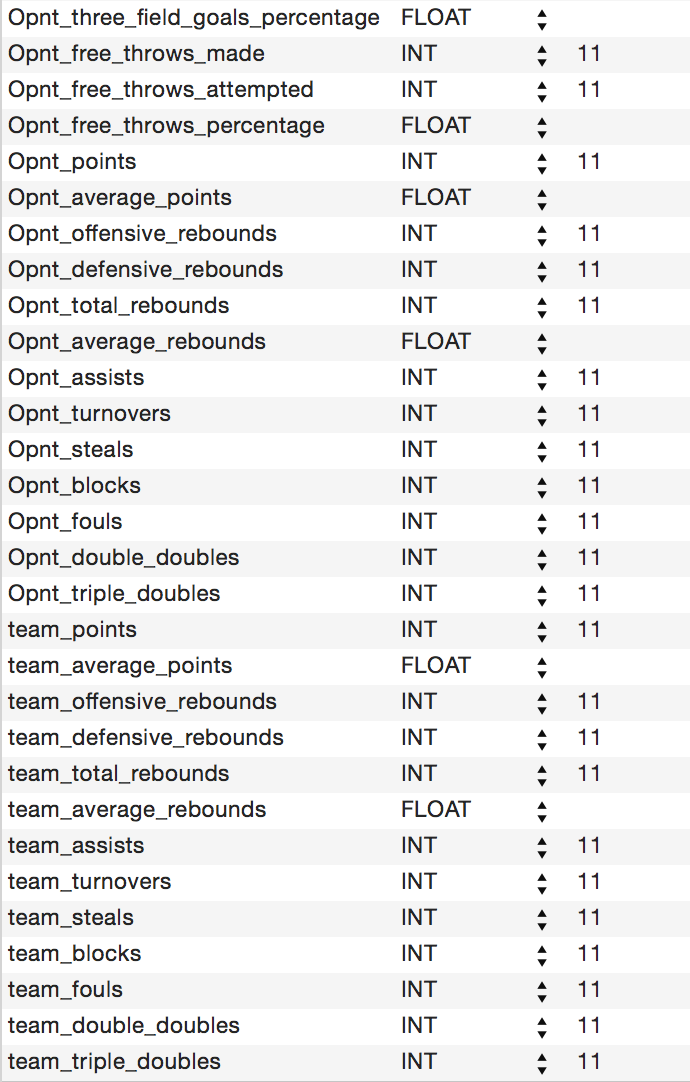
\includegraphics{SquadSeasonStat_table2.png}


\section{PlayerGameStat table}
\label{_static/database:playergamestat-table}
Contains the stats of one SquadMember in one Game

Many-to-one maps to SquadMember and many-to-one maps
to Game.

Table structure:

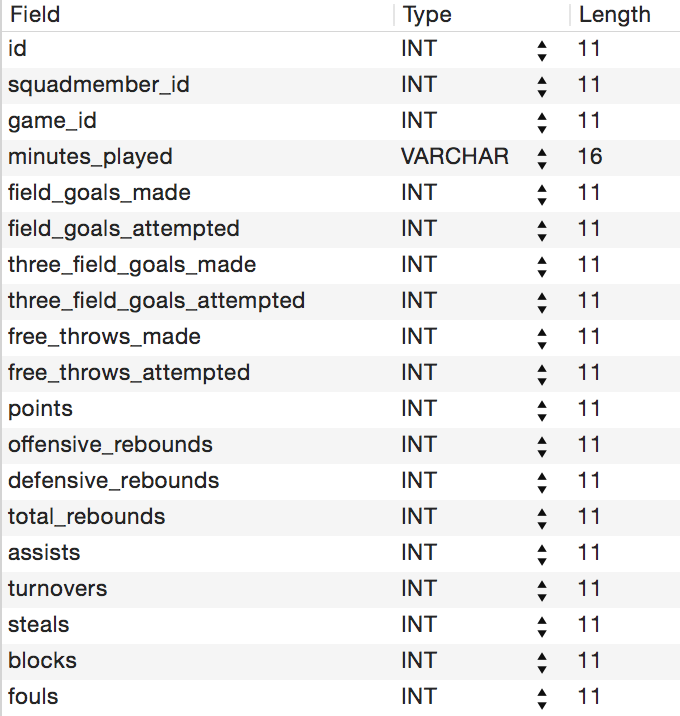
\includegraphics{PlayerGameStat_table.png}


\section{SquadGameStat table}
\label{_static/database:squadgamestat-table}
Contains the stats of one Squad in one Game

Many-to-one maps to Squad and Game

Table structure:

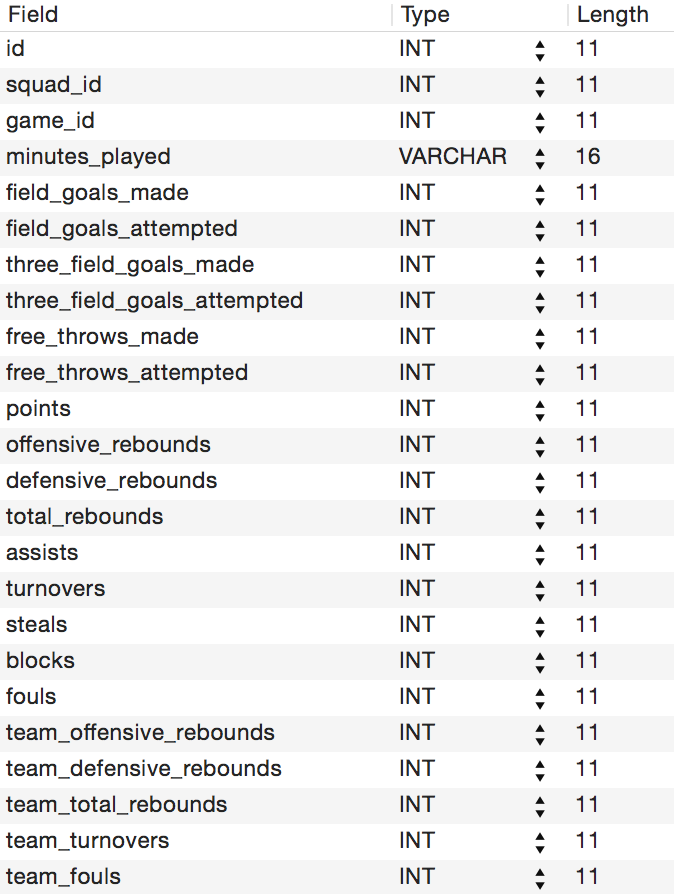
\includegraphics{SquadGameStat_table.png}


\section{GameDetail table}
\label{_static/database:gamedetail-table}
Play-by-Play information

Many-to-one maps to Game.

Table structure:

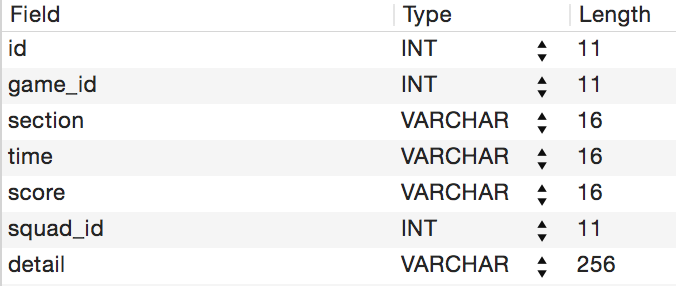
\includegraphics{GameDetail_table.png}


\chapter{How To Use}
\label{_static/howto:how-to-use}\label{_static/howto::doc}
This page provides simple use case for how to use this tool in backend.


\section{Command Line Interface}
\label{_static/howto:command-line-interface}
There are two CLIs for this project.

scheduler.py has 4 arguments to control the process:
\begin{enumerate}
\item {} 
-g \textless{}gender\textgreater{}: Use `men' or `women'

\item {} 
-t \textless{}type\textgreater{}: Use'new' or `initial'. If this is your first time to run this app and would like to get a full database of NCAA, use `initial'. If you already created a database but want to update it with newest data, use `new'.

\item {} 
-p \textless{}process\textgreater{}

\item {} 
-s \textless{}season\textgreater{}

\end{enumerate}

fix.py:
\begin{enumerate}
\item {} 
Item 1

\item {} 
Item 2

\end{enumerate}
\begin{description}
\item[{Usecase:}] \leavevmode\begin{itemize}
\item {} 
scheduler.py -g \textless{}gender\textgreater{} -t \textless{}type\textgreater{} -p \textless{}process\textgreater{} -s \textless{}season\textgreater{}

\item {} 
fix.py -g \textless{}gender\textgreater{} -p \textless{}process\textgreater{}

\end{itemize}

\end{description}


\section{Schedule of Cron Entries}
\label{_static/howto:schedule-of-cron-entries}
Words can have \emph{emphasis in italics} or be \textbf{bold} and you can define
code samples with back quotes, like when you talk about a command: \code{sudo}
gives you super user powers!


\chapter{Other Resources}
\label{index:other-resources}\begin{itemize}
\item {} 
\DUspan{xref,std,std-ref}{genindex}

\item {} 
\href{http://www.crummy.com/software/BeautifulSoup/bs4/doc/}{Beautiful Soup}

\item {} 
\DUspan{xref,std,std-ref}{search}

\end{itemize}



\renewcommand{\indexname}{Index}
\printindex
\end{document}
